\chapter{Реализация алгоритма}
\section{Предлагаемая схема параллелизации}
Две основные процедуры в алгоритме Фортена с модификацией Буздалова --- $NDHelperA$ и $NDHelperB$. Процедура $NDHelperA$ делит задачу на подзадачи и сливает результаты воедино посредством $NDHelperB$. Процедура $NDHelperB$ сама по себе является рекурсивной, следующей парадигме <<разделяй и властвуй>>. Деление задач происходит до момента, когда размерность $k$ станет равна $2$, что в дальнейшем обрабатывается отдельными процедурами.

Можно заметить, что на момент вызова процедуры $NDHelperB(L, H, k)$ ранги точек из множества $L$ уже вычислены и в дальнейшем меняться не будут. Также заметим, что порядок вызова подзадач в теле $NDHelperB$ не нарушит корректности алгоритма. Более того, мы можем разделить множество $L$ на любое количество частей ${L_1, L_2,\ldots, L_n}$ и тогда результат исполнения $NDHelperB(L_i, H, k)$ для всех $i$ будет идентичен результату исполнения $NDHelperB(L, H, k)$. Таким образом, $NDHelperB$ допускает параллельное исполнение.

С параллелизацией процедуры $NDHelperA$ возникают сложности. Внутренние вызовы $NDHelperA$ и $NDHelperB$ зависят друг от друга и имеют строго определенную последовательность. 

\section{Детали реализации}
Алгоритм был реализован на языке программирования Java с использованием Fork/Join фреймворка, который хорошо подходит для распараллеливания рекурсивных задач.

\begin{table}[h]
\caption{Сравнение времени работы алгоритмов при $N=10^4$}\label{tab1}
\centering
\begin{tabu}{|*{7}{c|}}
\hline
 & \multicolumn{3}{c|}{Original} & \multicolumn{3}{c|}{Parallel}\\
\cline{2-7}
M & min & max & avg & min & max & avg\\
\hline
3 & 2.40e+01 & 2.45e+01 & 2.42e+01 & 1.05e+02 & 1.14e+02 & 1.10e+02\\ 
4 & 9.14e+01 & 1.52e+02 & 9.60e+01 & 1.71e+02 & 2.19e+02 & 1.84e+02\\
5 & 2.06e+02 & 2.66e+02 & 2.14e+02 & 2.52e+02 & 2.75e+02 & 2.59e+02\\
6 & 3.44e+02 & 4.62e+02 & 3.62e+02 & 3.18e+02 & 3.46e+02 & 3.28e+02\\
7 & 4.64e+02 & 5.78e+02 & 4.92e+02 & 3.65e+02 & 3.93e+02 & 3.76e+02\\
8 & 5.43e+02 & 6.66e+02 & 5.74e+02 & 3.91e+02 & 4.28e+02 & 4.03e+02\\
9 & 5.74e+02 & 6.90e+02 & 6.03e+02 & 3.95e+02 & 4.33e+02 & 4.11e+02\\
10& 5.93e+02 & 7.55e+02 & 6.37e+02 & 4.03e+02 & 4.40e+02 & 4.19e+02\\
11& 6.03e+02 & 7.33e+02 & 6.46e+02 & 4.11e+02 & 4.43e+02 & 4.23e+02\\
12& 5.95e+02 & 7.91e+02 & 6.44e+02 & 4.14e+02 & 4.36e+02 & 4.24e+02\\
13& 5.92e+02 & 7.23e+02 & 6.41e+02 & 4.11e+02 & 4.36e+02 & 4.22e+02\\
14& 5.98e+02 & 7.35e+02 & 6.42e+02 & 4.07e+02 & 4.37e+02 & 4.23e+02\\
15& 5.98e+02 & 6.86e+02 & 6.30e+02 & 4.11e+02 & 4.35e+02 & 4.22e+02\\
\hline
\end{tabu}
\end{table}

\begin{figure}[h]
\centering
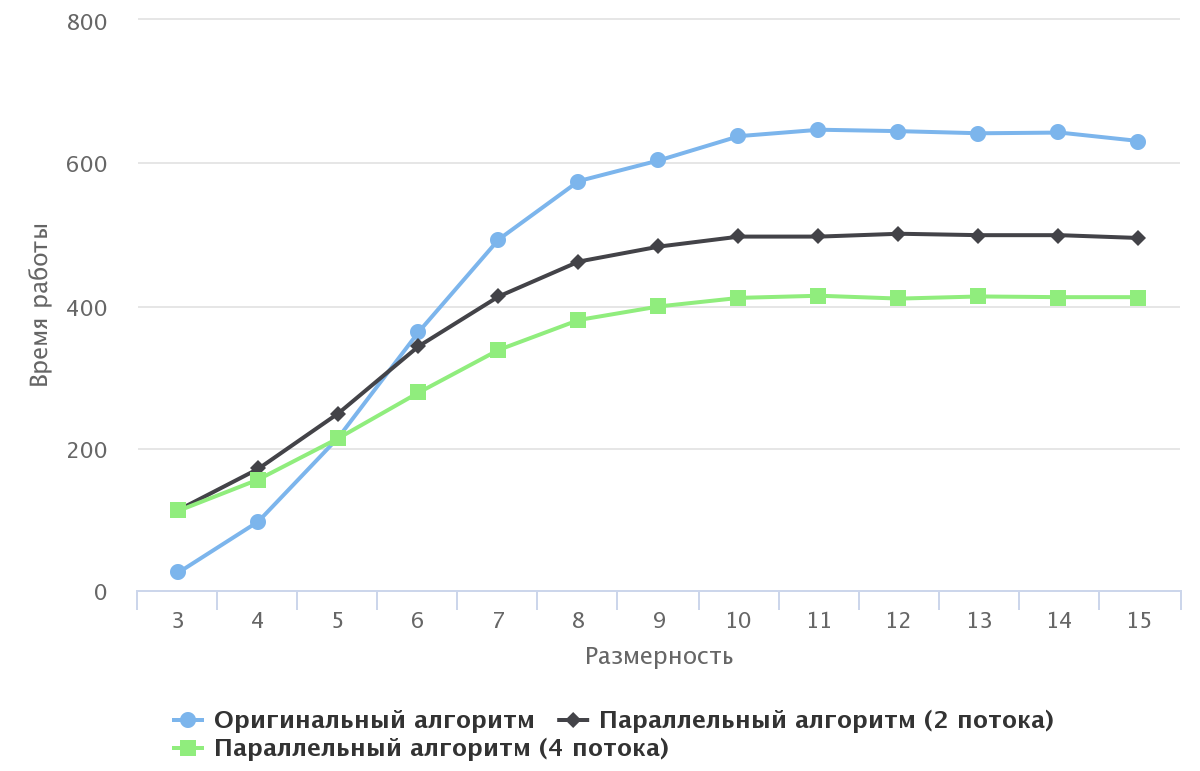
\includegraphics[width=0.9\textwidth]{images/10k.png}
\caption{Среднее время работы при $N=10^4$}
\label{pic1}
\end{figure}


\begin{table}[h]
\caption{Сравнение времени работы алгоритмов при $N=5\cdot10^4$}\label{tab2}
\centering
\begin{tabu}{|*{7}{c|}}
\hline
 & \multicolumn{3}{c|}{Original} & \multicolumn{3}{c|}{Parallel}\\
\cline{2-7}
M & min & max & avg & min & max & avg\\
\hline
3 & 1.63e+02 & 1.69e+02 & 1.64e+02 & 5.47e+02 & 5.72e+02 & 5.60e+02\\ 
4 & 6.88e+02 & 7.75e+02 & 7.05e+02 & 7.78e+02 & 8.45e+02 & 8.12e+02\\
5 & 1.73e+03 & 1.96e+03 & 1.82e+03 & 1.29e+03 & 1.34e+03 & 1.32e+03\\
6 & 3.23e+03 & 3.52e+03 & 3.39e+03 & 1.98e+03 & 2.06e+03 & 2.02e+03\\
7 & 4.99e+03 & 5.40e+03 & 5.16e+03 & 2.76e+03 & 2.91e+03 & 2.81e+03\\
8 & 6.44e+03 & 6.90e+03 & 6.65e+03 & 3.31e+03 & 3.47e+03 & 3.40e+03\\
9 & 7.40e+03 & 8.09e+03 & 7.68e+03 & 3.80e+03 & 4.04e+03 & 3.87e+03\\
10& 7.77e+03 & 8.51e+03 & 8.08e+03 & 4.05e+03 & 4.21e+03 & 4.12e+03\\
11& 7.95e+03 & 8.69e+03 & 8.33e+03 & 4.12e+03 & 4.34e+03 & 4.20e+03\\
12& 8.20e+03 & 8.77e+03 & 8.47e+03 & 4.16e+03 & 4.58e+03 & 4.25e+03\\
13& 8.10e+03 & 8.71e+03 & 8.34e+03 & 4.15e+03 & 6.00e+03 & 4.26e+03\\
14& 8.02e+03 & 8.61e+03 & 8.29e+03 & 4.13e+03 & 4.31e+03 & 4.20e+03\\
15& 8.03e+03 & 8.59e+03 & 8.36e+03 & 4.14e+03 & 4.30e+03 & 4.22e+03\\
\hline
\end{tabu}
\end{table}

\begin{figure}[h]
\centering
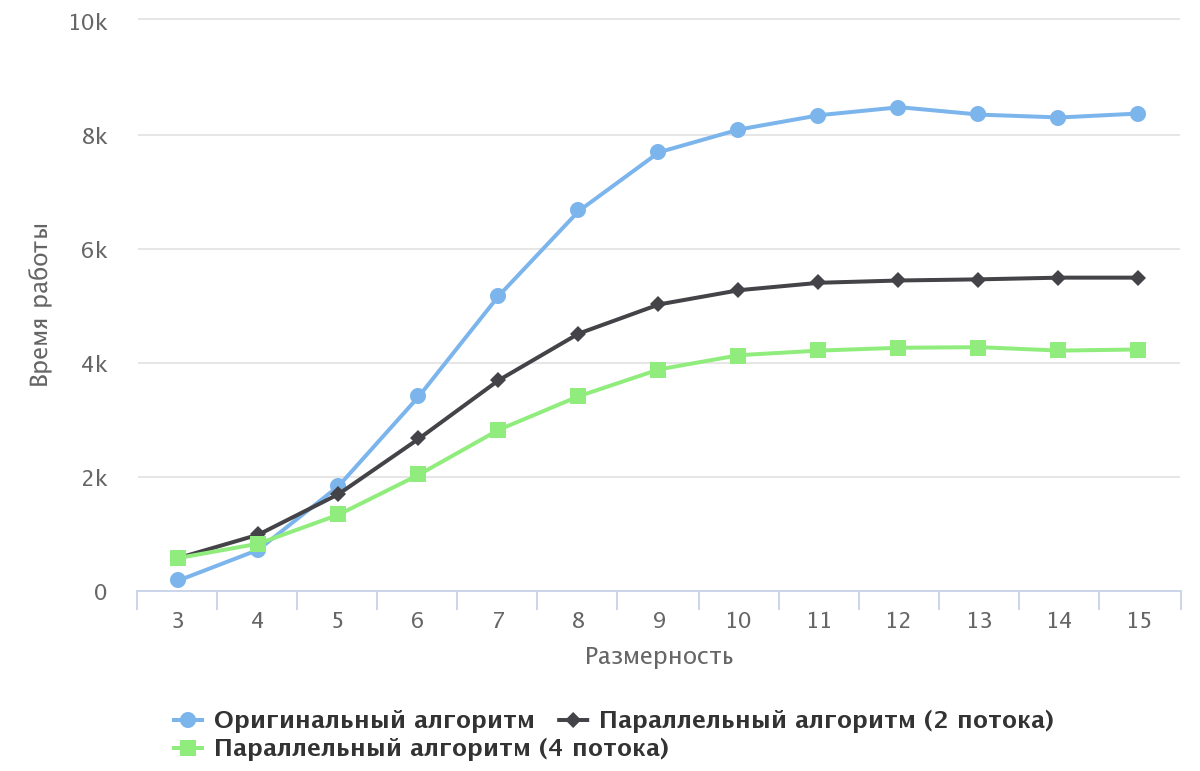
\includegraphics[width=0.9\textwidth]{images/50k.png}
\caption{Среднее время работы при $N=5*10^4$}
\label{pic2}
\end{figure}


\begin{table}[h]
\caption{Сравнение времени работы алгоритмов при $N=10^5$}\label{tab3}
\centering
\begin{tabu}{|*{7}{c|}}
\hline
 & \multicolumn{3}{c|}{Original} & \multicolumn{3}{c|}{Parallel}\\
\cline{2-7}
M & min & max & avg & min & max & avg\\
\hline
3 & 3.91e+02 & 3.97e+02 & 3.93e+02 & 1.16e+03 & 1.22e+03 & 1.18e+03\\ 
4 & 1.64e+03 & 1.71e+03 & 1.66e+03 & 1.71e+03 & 1.98e+03 & 1.74e+03\\
5 & 4.27e+03 & 4.57e+03 & 4.42e+03 & 2.92e+03 & 3.13e+03 & 2.98e+03\\
6 & 8.54e+03 & 8.97e+03 & 8.72e+03 & 4.79e+03 & 4.94e+03 & 4.85e+03\\
7 & 1.35e+04 & 1.51e+04 & 1.38e+04 & 6.95e+03 & 7.16e+03 & 7.04e+03\\
8 & 1.81e+04 & 2.38e+04 & 1.87e+04 & 8.95e+03 & 9.55e+03 & 9.18e+03\\
9 & 2.17e+04 & 2.25e+04 & 2.21e+04 & 1.05e+04 & 1.07e+04 & 1.06e+04\\
10& 2.34e+04 & 2.45e+04 & 2.39e+04 & 1.14e+04 & 1.17e+04 & 1.15e+04\\
11& 2.41e+04 & 2.52e+04 & 2.46e+04 & 1.17e+04 & 1.22e+04 & 1.19e+04\\
12& 2.46e+04 & 2.53e+04 & 2.49e+04 & 1.19e+04 & 1.23e+04 & 1.20e+04\\
13& 2.45e+04 & 2.57e+04 & 2.51e+04 & 1.18e+04 & 1.22e+04 & 1.20e+04\\
14& 2.44e+04 & 2.58e+04 & 2.51e+04 & 1.18e+04 & 1.23e+04 & 1.20e+04\\
15& 2.39e+04 & 2.52e+04 & 2.45e+04 & 1.20e+04 & 1.24e+04 & 1.22e+04\\
\hline
\end{tabu}
\end{table}

\begin{figure}[h]
\centering
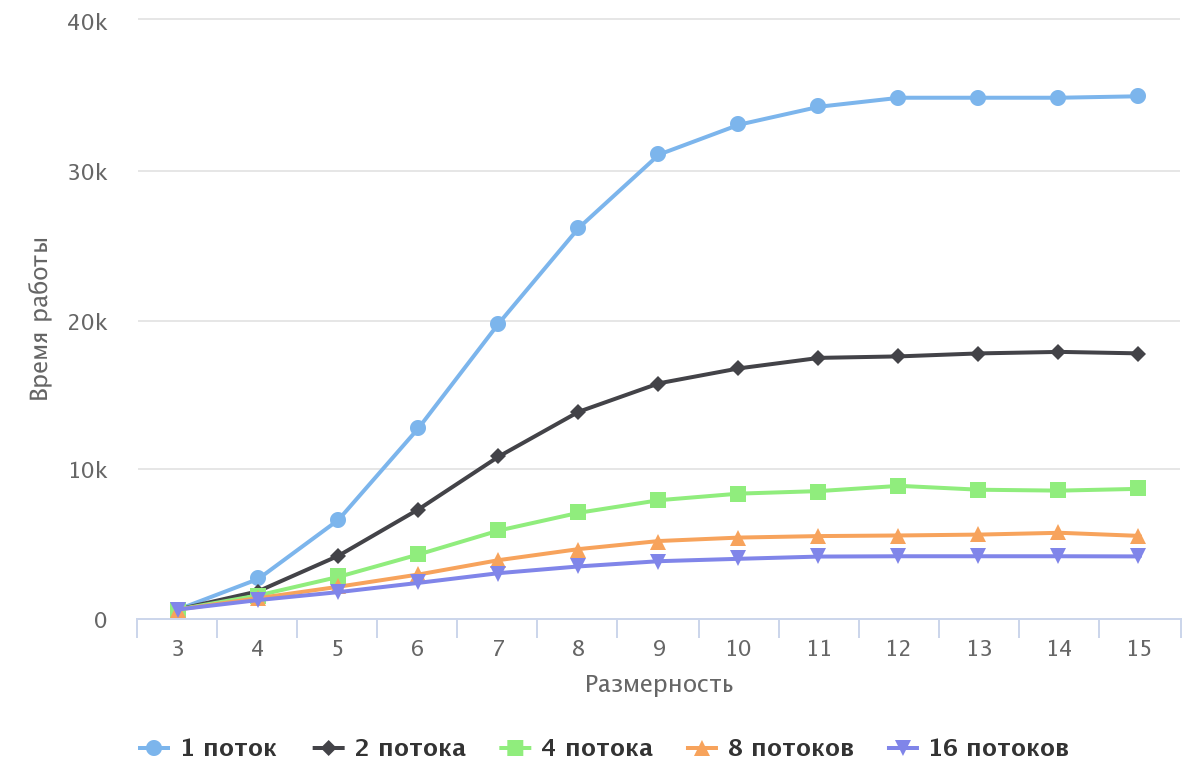
\includegraphics[width=0.9\textwidth]{images/100k.png}
\caption{Среднее время работы при $N=10^5$}
\label{pic3}
\end{figure}

